\documentclass[conference]{IEEEtran}
\IEEEoverridecommandlockouts

\usepackage{cite}
\usepackage{amsmath,amssymb,amsfonts}
% \usepackage{algorithmic}
\usepackage{graphicx}
\usepackage{textcomp}
\usepackage{xcolor}
\usepackage[hyphens]{url}

\def\BibTeX{{\rm B\kern-.05em{\sc i\kern-.025em b}\kern-.08em
    T\kern-.1667em\lower.7ex\hbox{E}\kern-.125emX}}


% \usepackage{graphicx}
% \usepackage{amsmath}
\usepackage{algorithm}
\usepackage[noend]{algpseudocode}
\usepackage{subcaption}
\usepackage{comment}
\usepackage{enumitem}
\usepackage{nameref}
 
\begin{document}

\pdfpagewidth=8.5in
\pdfpageheight=11in

\pagenumbering{arabic}

\title{MMA-Sim: Bit-Accurate Reference Model of Tensor Cores and Matrix Cores}
\author{Peichen Xie, Yang Wang, Fan Yang, Mao Yang\\\textit{Microsoft Research}}


\maketitle
\thispagestyle{plain}
\pagestyle{plain}


\begin{abstract}
The rapidly growing computation demands of deep neural networks (DNNs) have driven hardware vendors to integrate matrix multiplication accelerators (MMAs), such as NVIDIA Tensor Cores and AMD Matrix Cores, into modern GPUs. However, due to distinct and undocumented arithmetic specifications for floating-point matrix multiplication, some MMAs can lead to numerical imprecision and inconsistency that can compromise the stability and reproducibility of DNN training and inference.

This paper presents MMA-Sim, the first bit-accurate reference model that reveals the detailed arithmetic behaviors of the MMAs from ten GPU architectures (eight from NVIDIA and two from AMD). By dissecting the MMAs using a combination of targeted and randomized tests, our methodology derives nine arithmetic algorithms to simulate the floating-point matrix multiplication of the MMAs. Large-scale validation confirms bitwise equivalence between MMA-Sim and the real hardware. Using MMA-Sim, we investigate arithmetic behaviors that affect DNN training stability, and identify undocumented behaviors that could lead to significant errors.
    
\end{abstract}
\section{Introduction}

To satisfy the rapidly growing computation demands of deep neural networks (DNNs), hardware vendors have introduced specialized floating-point matrix multiplication accelerators (MMAs) in their latest GPU architectures. MMAs such as NVIDIA Tensor Cores \cite{markidis_nvidia_2018,sun_dissecting_2023} and AMD Matrix Cores \cite{schieffer_rise_2024} empower modern GPUs with PetaFLOPS-scale computing capability, and play a pivotal role in the training and inference of frontier DNNs such as large language models (LLMs).

However, the rapid evolution of these high-performance MMAs introduces new challenges because no publicly available document specifies the exact arithmetic for floating-point matrix multiplication (\S\ref{sec:motivation}).  
Recent studies \cite{deepseek-ai_deepseek-v3_2024,pytorch_developers_pytorch_2025} have shown that insufficient arithmetic precision and dynamic range in some MMAs can lead to unexpected degradation in DNN training accuracy, particularly for LLMs. Diagnosing and preventing this issue is challenging because the internal arithmetic behaviors of MMAs are typically undocumented and thus poorly understood.

Moreover, different vendors adopt diverse approaches for the same matrix multiplication operations, and diversity exists even between different generations of MMAs from the same vendor \cite{li_discovery_2024}. These variations lead to subtle, sometimes significant numerical inconsistencies in matrix multiplication results, and consequently compromise the reproducibility of higher-level DNN training and inference.

To address these challenges, this paper presents MMA-Sim, the first bit-accurate reference model that reveals the detailed arithmetic behaviors of matrix multiplication accelerators (MMAs). Given input matrices with specified data types and shapes, MMA-Sim produces an output matrix that matches the MMA’s output bit by bit. By faithfully modeling each MMA’s arithmetic behavior, MMA-Sim enables thorough understanding, transparent analysis, and bit-accurate simulation of the subtle arithmetic intricacies of the MMA. With MMA-Sim, software developers can diagnose and prevent numerical issues in precision-sensitive DNN training and inference, and hardware designers can design new MMAs with numerical consistency to established and widely-adopted MMAs.

Bit-accurate modeling of MMAs is non-trivial. Most MMAs are black boxes for the public, meaning that their arithmetic implementations are not disclosed. To uncover the detailed arithmetic behaviors of each matrix multiplication instruction of each MMA, we employ specially crafted inputs along with randomized inputs to detect the characteristics of the MMA in both edge and typical cases (\S\ref{sec:method}). Based on the observed results, we construct an arithmetic algorithm that models the arithmetic behavior of the instruction. The algorithm specifies the step-by-step computation procedure, including the operation type, operation order, rounding method, precision, and other implementation details. The correctness of each algorithm is carefully validated against the MMA output at the bit level, and iteratively refined until bitwise equivalence is achieved.

Applying this testing-based approach to all matrix multiplication instructions from ten GPU architectures, we construct nine arithmetic algorithms (\S\ref{sec:model}). Using the nine algorithms, we implement MMA-Sim using approximately 2800 lines of Python code. MMA-Sim faithfully simulates the diverse arithmetic of all floating-point matrix multiplication instructions across all the eight NVIDIA GPU architectures with Tensor Cores (from Volta to RTX Blackwell) and the two latest AMD GPU architectures with Matrix Cores (CDNA2 and CDNA3). MMA-Sim is validated against real hardware through extensive large-scale random testing (\S\ref{sec:correctness}). We test each instruction with more than one million sets of randomly generated input matrices, and the results confirm bitwise equivalence between MMA-Sim and the corresponding hardware.

Through MMA-Sim, we investigate previously reported issues and uncover many previously unknown characteristics in MMA designs across vendors and architectures (\S\ref{sec:findings}). For example, we confirm the reduced accumulation precision of the 8-bit floating-point (FP8) instructions on the NVIDIA Hopper architecture, and the reduced dynamic range of the 16-bit floating-point (FP16 and BF16) instructions on the AMD CDNA2 architecture, both of which can adversely affect DNN training, as reported in previous work \cite{deepseek-ai_deepseek-v3_2024,pytorch_developers_pytorch_2025}. We also discover the reduced accumulation precision of the FP8 instructions on the NVIDIA Ada Lovelace architecture, and find that the precision is increased on the newer Blackwell and RTX Blackwell architectures. Moreover, we identify the asymmetric rounding used in the TF32 (TensorFloat-32), FP16, and BF16 instructions on the AMD CDNA3 architecture, which can introduce notable numerical errors and biases in certain conditions. Interestingly, we also find that the rounding method has been specially modified in the FP8 instructions on the CDNA3 architecture, which mitigates such issues.

These findings demonstrate the power of MMA-Sim as an analytical tool to understand the detailed arithmetic behaviors of modern accelerators. For software developers, MMA-Sim bridges the gap between hardware implementations and software expectations, and enables systematic investigation of numerical error sources, stability analysis of training algorithms, and hardware-specific precision tuning. For hardware designers, MMA-Sim as a bit-accurate reference model captures the full spectrum of arithmetic subtleties, providing the detailed functional specifications for future MMA design and verification.


In summary, this paper makes the following contributions.

\begin{itemize}
\item Systematically dissecting MMA arithmetic behaviors. We develop a testing-based methodology that detects each MMA’s arithmetic behavior through specially crafted inputs and random inputs, and derive nine distinct arithmetic algorithms that capture their arithmetic for floating-point matrix multiplication.
\item Bit-accurate reference model. We present MMA-Sim, the first bit-accurate reference model that simulates the exact arithmetic behaviors of modern MMAs across vendors and architectures with the nine arithmetic algorithms.
\item Implementation and validation. We implement MMA-Sim for ten GPU architectures (eight from NVIDIA and two from AMD) and validate its correctness via large-scale random testing, confirming bitwise equivalence with the real hardware.
\item New insights into MMA arithmetic design and usage. Through MMA-Sim, we identify many undocumented design choices that explain the reported instability in DNN training or introduce new numerical issues, and we suggest mitigation approaches to both hardware and software developers.
\item Practical analytical utility. MMA-Sim will be open-source, providing a unified framework for MMA arithmetic behavior modeling, numerical analysis, arithmetic design specification, and hardware-aware optimization in both software and hardware design.
\end{itemize}

\section{Motivation}
\label{sec:motivation}

Floating-point matrix multiplication is the most computationally intensive operation in modern deep neural networks (DNNs), especially in large language models (LLMs). To accelerate floating-point matrix multiplication, modern GPUs have integrated specialized matrix multiplication accelerators (MMAs) such as NVIDIA Tensor Cores and AMD Matrix Cores. MMAs provide various matrix multiplication instructions (MMIs) that accelerate one or more matrix multiply-add operations
\begin{equation}
\label{eq:mm}
D_{M\times N} = A_{M\times K} \times B_{K\times N} + C_{M\times N},
\end{equation} 
where $A$, $B$, and $C$ are input matrices, and $D$ is the output matrix. $C$ and $D$ serve as accumulators so that large matrix multiplications can be computed by iterating the matrix multiply-add operations. For example, multiplying two $64\times 64$ matrices requires $(64/M)\times (64/N)\times (64/K)$ matrix multiply-add operations.

However, the complexity and diversity of MMIs introduce numerical issues that have profound implications for DNNs. As there is currently no specification that standardizes the design and arithmetic behavior of MMIs, hardware vendors can implement the MMIs at their own discretion. As a result, different vendors provide MMIs with different shapes and data types, as detailed in the \nameref{sec:appendix}. Although some MMIs retain the same shapes and data types across several generations of MMAs from the same vendor, previous studies \cite{fasi_numerical_2021,li_fttn_2024,xie_revealing_2025} have revealed that different generations of MMAs adopt distinct approaches for computing the same matrix multiply-add operation (Equation \ref{eq:mm}).

Specifically, since no specification defines the standard output of Equation \ref{eq:mm}, hardware vendors are free to implement it with different computational precision, dynamic ranges, rounding modes, special-value handling rules, etc. These implementation details are undocumented, but they are critical to the numerical accuracy of matrix multiplication and higher-level DNNs. For example, previous studies \cite{deepseek-ai_deepseek-v3_2024,pytorch_developers_pytorch_2025} have reported that the accumulation precision of 8-bit floating-point (FP8) MMIs on the NVIDIA Hopper architecture and the dynamic range of 16-bit floating-point (FP16 and BF16) MMIs on the CDNA2 architecture are insufficient for stable DNN training, and can lead to significant degradation in training accuracy. As the root cause is the undocumented internal arithmetic behavior of the hardware, it is difficult for software developers to diagnose and address the issues.

In addition, as MMIs differ in shape and arithmetic behavior, different MMAs will produce inconsistent outputs for the same floating-point matrix multiplication \cite{li_discovery_2024}. Consequently, the reproducibility of DNNs is compromised, and maintaining consistent DNN behaviors across different MMAs becomes very difficult. Without understanding the arithmetic behaviors of existing MMAs, it is also difficult for new hardware vendors to ensure numerical consistency with them.

Therefore, complete and accurate modeling of the arithmetic behaviors of MMAs is crucial for addressing these issues. To this end, we aim to construct a bit-accurate reference model for MMAs, which provides a thorough dissection and bit-accurate simulation of the arithmetic behavior of each MMI.

\section{Methodology}
\label{sec:method}

\subsection{Workflow overview}

A bit-accurate reference model is an executable behavior model that is bitwise equivalent to the arithmetic behavior of the corresponding hardware. For each matrix multiplication accelerator (MMA) and each matrix multiplication instruction (MMI), the bit-accurate reference model provides an arithmetic algorithm $f$ such that
\begin{equation}
    f(A,B,C) = \mathrm{MMI}_{\mathrm{MMA}}(A,B,C),
\end{equation}
given any input matrices $A$, $B$, and $C$ with the shape and data type specified by the MMI.

To build this bit-accurate reference model, we adopt a testing-based, non-intrusive approach, treating the hardware behavior as a black box. Specifically, for each generation of Tensor Cores and Matrix Cores, we examine each MMI, and build an arithmetic algorithm $f$ for the MMI following the workflow shown below.

\begin{enumerate}
    \item First, we construct specially crafted inputs to test the MMI, and detect the characteristics of the MMI according to its output on the MMA. The characteristics include summation order, accumulation precision, rounding modes, special value handling rules, etc.
    \item Based on the detected characteristics, we construct an algorithm to compute Equation \ref{eq:mm}, and implement this algorithm with Python.
    \item Then, we validate the correctness of the algorithm by comparative testing. Given over a million sets of random inputs, if the outputs of our algorithm are bitwise consistent with the outputs of hardware, we stop here and examine the next MMI.
    \item Otherwise, we analyze the differences in the outputs and refine our algorithm accordingly to fix the mismatch. The test and refinement are repeated until the validation succeeds.
\end{enumerate}

In the remainder of this section, we first show that modeling the matrix multiply-add operation of MMIs can be simplified to modeling the dot-add operation. Then, we introduce the main characteristics we test and how we design special inputs for them.

\subsection{Problem simplification}

We first check whether each element of the output matrix $D$ is computed in the same way---that is, whether the dot-add computation 
\begin{equation}
\label{eq:dij}
    d_{ij} = c_{ij}+\sum_{k=0}^{K-1} a_{ik}b_{kj}
\end{equation}
depends on the indices $i$ and $j$. To test this, we first set $i=0$ and $j=0$ and generate random inputs $a_{0k}$, $b_{k0}$, and $c_{00}$ for $k=0,1,...,K-1$. Then, we set $a_{ik}=a_{0k}$, $b_{kj}=b_{0j}$, and $c_{ij}=c_{00}$ for all other $i$ and $j$. By sending the input to the MMA, we see that each element $d_{ij}$ in the output is bitwise identical. We observe such consistent behavior across large-scale random tests. Therefore, each output element in $D$ is computed in the same way.

In the following part of this paper, we simplify the notation of Equation \ref{eq:dij} to
\begin{equation}
\label{eq:d}
\begin{split}
    d &= c + \sum_{k=0}^{K-1}a_{k}b_{k} \\
     &= f(c, a_0, a_1, ..., a_{K-1}, b_0, b_1, ..., b_{K-1}).
\end{split}
\end{equation}
Hence, our goal is reduced to building a $(2K+1)$-input algorithm $f(c, \mathbf{a}, \mathbf{b})$ for the dot-add computation of each MMI.

\subsection{Summation order}

We use specially crafted inputs to detect the summation order in the computation of Equation \ref{eq:d}. The inputs are constructed so that the $K+1$ summands
\begin{equation}
    p_k=\begin{cases}
        a_kb_k &\text{if $0\le k < K$} \\
        c &\text{if $k=K$}
    \end{cases}
\end{equation}
consist of a very large power of two $X$, its negation $-X$, and $K-1$ numbers with the same value $y$ that is a very small power of two. When sending such input to the MMA, the hardware output divided by $y$ represents the number of summands summed after the neutralization of $p_i+p_j=0$ where $p_i=X$ and $p_j=-X$, so we can determine the priority of the summation operation between $p_i$ and $p_j$. We run this numerical experiment with $X$ and $-X$ at different locations, so we can construct the summation tree based on the priority information. We construct the summation tree by leveraging the tree construction algorithms in \cite{xie_revealing_2025}.

As a result, we can generate a summation tree that represents the summation order. For example, Figure \ref{fig:tree} shows four typical summation trees that we construct for MMIs on all generations of Tensor Cores and Matrix Cores. 

\begin{figure}[ht]
\begin{subfigure}[b]{0.4\linewidth}
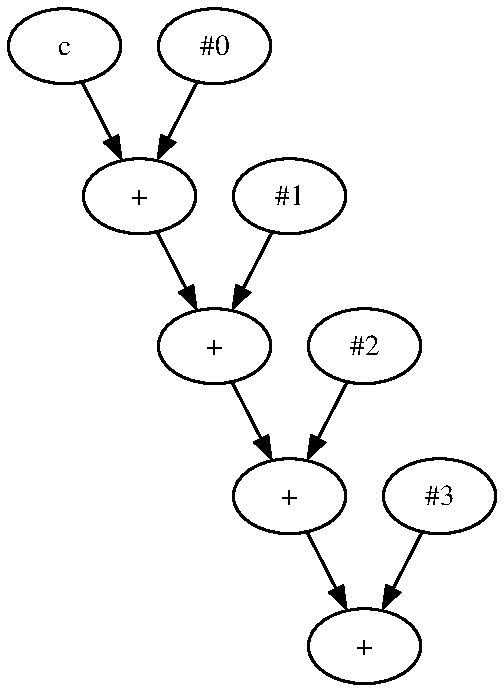
\includegraphics[width=0.8\linewidth]{figures/sequential.pdf}
\caption{Sequential summation.}
\end{subfigure}
\begin{subfigure}[b]{0.6\linewidth}
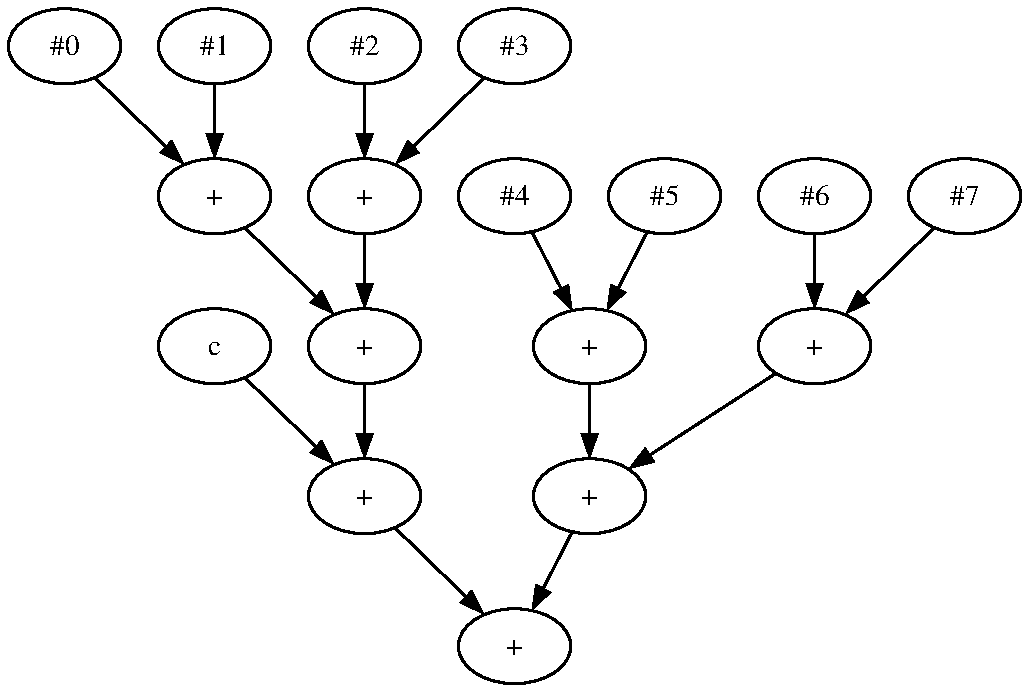
\includegraphics[width=1\linewidth]{figures/pairwise.pdf}
\caption{Group pairwise summation.}
\end{subfigure}
\begin{subfigure}[b]{0.4\linewidth}
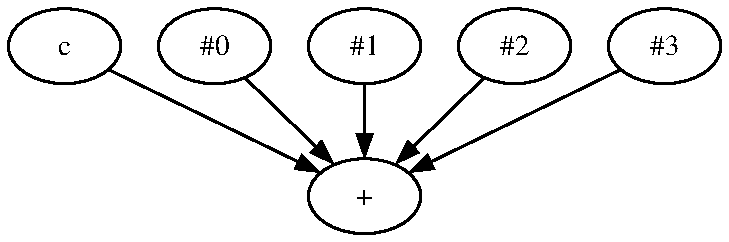
\includegraphics[width=1\linewidth]{figures/fused.pdf}
\caption{Fused summation.}
\end{subfigure}
\begin{subfigure}[b]{0.6\linewidth}
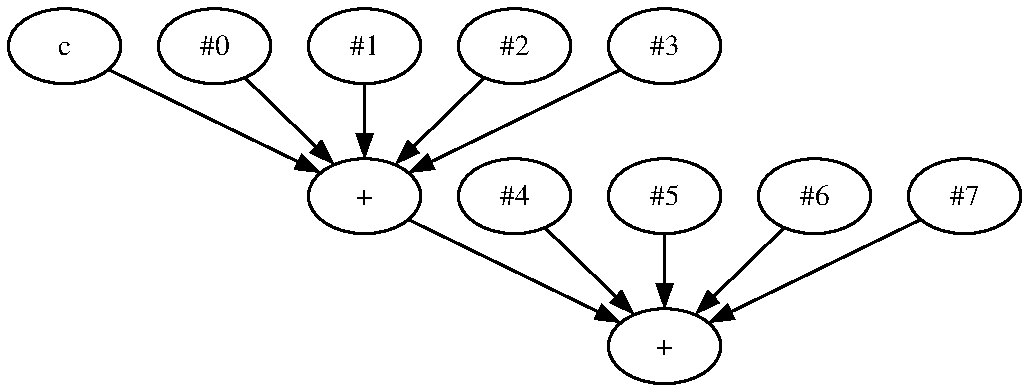
\includegraphics[width=1\linewidth]{figures/chain_of_fused.pdf}
\caption{Chain of fused summations.}
\end{subfigure}
\caption{Four typical summation orders on Tensor Cores and Matrix Cores. \#$i$ represents the product $a_ib_i$.}
\label{fig:tree}
\end{figure}

The first two summation trees are binary trees, representing that the summation is composed of binary addition operations with different orders. Figure \ref{fig:tree}(a) shows the summation tree of the DMMA.884 instruction on the Ampere architecture, indicating the sequential summation order. Figure \ref{fig:tree}(b) shows the summation tree of the v\_mfma\_f32\_32x32x8\_f16 instruction on the CDNA2 architecture, indicating the pairwise summation order within groups of four summands and the sequential summation order among $c$ and the group sums. 

The last two summation trees are multiway trees. A $t$-ary tree represents that the summation is based on $t$-term fused summation, which means that the $t$ terms are summed before the intermediate summation result is normalized to the floating-point number. Figure \ref{fig:tree}(c) shows the summation tree of the HMMA.1684.F32.TF32 instruction on the Ampere architecture, indicating that the 5-term fused summation is used. Figure \ref{fig:tree}(d) shows the summation tree of the HMMA.1688.F32.TF32 instruction on the Ampere architecture, indicating that two five-term fused summations are used iteratively.

\subsection{Accumulation precision}

We use specially crafted inputs to detect the precision in the summation of Equation \ref{eq:d}. For each summation based on binary addition operations, we use $1.0 + \epsilon$ to test its precision. Specifically, for the summation of $p_i$ and $p_j$, we first set $p_i=1.0$ and $p_j=\epsilon=1.0$, and set other summands to zero. Next, we repeatedly halve $\epsilon$ until the hardware output satisfies $d\neq 1.0+\epsilon$. Then, we conclude that the accumulation precision of $p_j$ in this operation is $1-\log_2 \epsilon$ bits after the radix point. We can determine the precision of all summands in all addition operations by running this numerical experiment with different $i$ and $j$ indices.

For each $t$-term fused summation, we use $-1.0+1.0+\epsilon$ to test the precision of the operation. Similarly, for the summation operation including $p_i$, $p_j$, and $p_k$, we first set $p_i=-1.0$, $p_j=1.0$, and $p_k=\epsilon=1.0$, and set other summands to zero. Next, we continuously halve $\epsilon$ until the hardware output $d\neq \epsilon$. Then, we conclude that the precision of $p_k$ is $1-\log_2 \epsilon$ bits after the radix point. We can determine the precision of all summands in all summation operations by running this numerical experiment with different $i$, $j$, and $k$ indices.

\subsection{Rounding mode}

After detecting the accumulation precision, we analyze the rounding mode for each summation operation by specially crafted inputs. We first set the unit in the last place $u=2\epsilon$. Then, we construct the input to make the unrounded sum equal to $1.0+0.75u$, $1.0+0.25u$, $-1.0-0.75u$, and $-1.0-0.25u$. According to the rounded results, we refer to Table \ref{tab:rounding} and identify the rounding mode, which can be rounding up (RU), rounding down (RD), rounding to zero (RZ), rounding away from zero (RA), or rounding to nearest (RN).

\begin{table}[ht]
\caption{Rounding mode detection according the rounding results of four inputs.}
\label{tab:rounding}
\centering
\begin{tabular}{|l|l|l|l|l|}
\hline
Input & $1+0.75u$ & $1+0.25u$ & $-1-0.75u$ & $-1-0.25u$ \\ \hline
RU & $1+u$ & $1+u$ & $-1$ & $-1$ \\ \hline
RD & $1$ & $1$ & $-1-u$ & $-1-u$ \\ \hline
RZ & $1$ & $1$ & $-1$ & $-1$ \\ \hline
RA & $1+u$ & $1+u$ & $-1-u$ & $-1-u$ \\ \hline
RN & $1+u$ & $1$ & $-1-u$ & $-1$ \\ \hline
\end{tabular}
\end{table}

If the rounding mode belongs to RN, we further test $1.0+0.5u$, $1.0+1.5u$, $-1.0-0.5u$, and $-1.0-1.5u$. According to the rounded results, we refer to Table \ref{tab:rn} and identify the tie-breaking rule of RN, which can be rounding ties up (RNU), rounding ties down (RND), rounding ties to zero (RNZ), rounding ties away from zero (RNA), rounding ties to even (RNE), or rounding ties to odd (RNO).

\begin{table}[ht]
\caption{Tie-breaking rule detection for rounding-to-nearest modes according the rounding results of four inputs.}
\label{tab:rn}
\centering
\begin{tabular}{|l|l|l|l|l|}
\hline
Input & $1+0.5u$ & $1+1.5u$ & $-1-0.5u$ & $-1-1.5u$ \\ \hline
RNU & $1+u$ & $1+u$ & $-1$ & $-1-u$ \\ \hline
RND & $1$ & $1+u$ & $-1-u$ & $-1-2u$ \\ \hline
RNZ & $1$ & $1+u$ & $-1$ & $-1-u$ \\ \hline
RNA & $1+u$ & $1+2u$ & $-1-u$ & $-1-2u$ \\ \hline
RNE & $1$ & $1+2u$ & $-1$ & $-1-2u$ \\ \hline
RNO & $1+u$ & $1+u$ & $-1-u$ & $-1-u$ \\ \hline
\end{tabular}
\end{table}

\subsection{Special value handling}

Subnormal numbers, negative zero, infinity, and NaNs are special values in floating-point arithmetic. We construct inputs in edge conditions to detect the special value handling rules of the MMI.

For subnormal numbers, we first set $c$ to $0.5\epsilon$ (where $\epsilon$ is the smallest positive normal number) and set other inputs to zero. If the hardware output equals zero, it indicates that the subnormal input of $c$ is flushed to zero. Similarly, we set an input $a_k$ (or $b_k$) to $0.5\epsilon$, set the corresponding $b_k$ (or $a_k$) to one, and set other inputs to zero. If the hardware output equals zero, it indicates that the subnormal input of $a_k$ (or $b_k$) is flushed to zero. Next, we detect whether subnormal values will be flushed after multiplication by setting an input $a_k=0.5$, setting its corresponding $b_k=\epsilon$, and setting other inputs to zero. Finally, we detect whether subnormal values will be flushed after addition by setting a summand $p_i=1.5\epsilon$, setting another summand $p_j=-\epsilon$, and setting other inputs to zero.

For negative zeros, we detect whether a negative zero can be generated by setting the inputs to $-0.0+\sum_{k=0}^{K-1}(+0.0)\times(-0.0)$. Whether the hardware output equals $-0.0$ indicates whether the negative zero can be generated.

For infinity, we detect whether multiplication can overflow by setting $a_k=2.0$ for some $k$, setting $b_k=2^E$, $c=-2^E$, and setting other inputs to zero, where $E$ is the maximum exponent of the input floating-point format. We also detect whether intermediate summation can overflow by testing $2^E+2^E-2^E$. Then, we detect the rules for overflows by testing the edge conditions $(2-u)\times2^E+0.75u\times2^E$, $(2-u)\times2^E+0.5u\times2^E$, $(2-u)\times2^E+0.25u\times2^E$, $(-2+u)\times2^E-0.75u\times2^E$, $(-2+u)\times2^E-0.5u\times2^E$, and $(-2+u)\times2^E-0.25u\times2^E$.

For NaNs, we set $p_k=0.0\times\infty$ for some $k$, and set other inputs to zero; then we set $p_i=-\infty$ and $p_j=+\infty$ for some $i$ and $j$, and set other inputs to zero. We find that NaNs can be generated in both cases for all the tested MMAs.
\section{Bit-Accurate Reference Model}
\label{sec:model}

Based on our numerical experiments for the matrix multiplication instructions (MMIs) from ten GPU architectures, including all the eight NVIDIA GPU architectures with Tensor Cores (from Volta to RTX Blackwell) and the latest two AMD architectures with Matrix Cores (CDNA2 and CDNA3), we construct nine arithmetic algorithms in total. Table \ref{tab:nvmodel} lists our arithmetic algorithms for Tensor Core instructions, and Table \ref{tab:amdmodel} lists our arithmetic algorithms for Matrix Core instructions.

Based on these arithmetic algorithms, we build a simulator called MMA-Sim, which serves as our bit-accurate reference model. With MMA-Sim, users can simulate any MMI from any GPU architecture by providing input floating-point matrices $A$, $B$, and $C$, and obtain the output matrix $D$ such that $d_{ij}=f(c_{i,j}, a_{i0}, a_{i1}, ..., b_{0j}, b_{1j}, ...)$ where $f$ is the arithmetic algorithm for the MMI.

\begin{table*}[t]
\caption{Bit-accurate arithmetic algorithms for NVIDIA Tensor Core instructions on eight architectures from Volta to RTX Blackwell. Each cell shows the algorithm that models the instruction bit-accurately. N/A means the instruction is not available for the architecture.}
\label{tab:nvmodel}
\centering \scriptsize
\begin{tabular}{|l|l|l|l|l|l|l|l|}
\hline
Instruction & Volta & Turing & Ampere & Ada Lovelace & Hopper & Blackwell & RTX Blackwell \\ \hline
\begin{tabular}[c]{@{}l@{}}HMMA.884.F32.F32\\ HMMA.884.F32.F16\\ HMMA.884.F16.F16\end{tabular} & FDA(F=23) & FDA(F=24) & N/A & N/A & N/A & N/A & N/A \\ \hline
\begin{tabular}[c]{@{}l@{}}HMMA.1688.F32\\ HMMA.1688.F16\end{tabular} & N/A & FDA(F=24) & FDA(F=24) & FDA(F=24) & FDA(F=25) & FDA(F=25) & FDA(F=25) \\ \hline
DMMA.884 / DMMA.8x8x4 & N/A & N/A & SFMA & SFMA & SFMA & SFMA & SFMA \\ \hline
\begin{tabular}[c]{@{}l@{}}HMMA.1688.F32.TF32\\ HMMA.16816.F32\\ HMMA.16816.F16\\ HMMA.16816.F32.BF16\end{tabular} & N/A & N/A & CoFDA(F=24) & CoFDA(F=24) & FDA(F=25) & FDA(F=25) & FDA(F=25) \\ \hline
\begin{tabular}[c]{@{}l@{}}HMMA.1684.F32.TF32\\ HMMA.1688.F32.BF16\end{tabular} & N/A & N/A & FDA(F=24) & FDA(F=24) & FDA(F=25) & FDA(F=25) & FDA(F=25) \\ \hline
\begin{tabular}[c]{@{}l@{}}QMMA.16832.F32.\textit{f8type}.\textit{f8type}\\ QMMA.16832.F16.\textit{f8type}.\textit{f8type}\end{tabular} & N/A & N/A & N/A & CoFDA(F=13) & N/A & N/A & FDA(F=25) \\ \hline
\begin{tabular}[c]{@{}l@{}}QMMA.16816.F32.\textit{f8type}.\textit{f8type}\\ QMMA.16816.F16.\textit{f8type}.\textit{f8type}\end{tabular} & N/A & N/A & N/A & FDA(F=13) & N/A & N/A & FDA(F=25) \\ \hline
\begin{tabular}[c]{@{}l@{}}DMMA.16x8x16\\ DMMA.16x8x8\\ DMMA.16x8x4\end{tabular} & N/A & N/A & N/A & N/A & SFMA & N/A & N/A \\ \hline
\begin{tabular}[c]{@{}l@{}}HGMMA.64x8x8.F32.TF32\\ HGMMA.64x8x16.F32\\ HGMMA.64x8x16.F16\\ HGMMA.64x8x16.F32.BF16\end{tabular} & N/A & N/A & N/A & N/A & FDA(F=25) & N/A & N/A \\ \hline
\begin{tabular}[c]{@{}l@{}}QGMMA.64x8x32.F32.\textit{f8type}.\textit{f8type}\\ QGMMA.64x8x32.F16.\textit{f8type}.\textit{f8type}\end{tabular} & N/A & N/A & N/A & N/A & FDA(F=13) & N/A & N/A \\ \hline
\begin{tabular}[c]{@{}l@{}}UTCHMMA\\ UTCQMMA\end{tabular} & N/A & N/A & N/A & N/A & N/A & FDA(F=25) & N/A \\ \hline
\begin{tabular}[c]{@{}l@{}}UTCOMMA\\ UTCOMMA.4X\end{tabular} & N/A & N/A & N/A & N/A & N/A & GDFS & N/A \\ \hline
\begin{tabular}[c]{@{}l@{}}QMMA.16832.F32.\textit{f8f6f4type}.\textit{f8f6f4type}\\ QMMA.16832.F16.\textit{f8f6f4type}.\textit{f8f6f4type}\\ QMMA.SF.16832.F32.\textit{f8f6f4type}.\textit{f8f6f4type}.E8\end{tabular} & N/A & N/A & N/A & N/A & N/A & N/A & FDA(F=25) \\ \hline
\begin{tabular}[c]{@{}l@{}}OMMA.SF.16864.F32.E2M1.E2M1.E8\\ OMMA.SF.16864.F32.E2M1.E2M1.UE4M3.4X\end{tabular} & N/A & N/A & N/A & N/A & N/A & N/A & GDFS \\ \hline
\end{tabular}
\\
\footnotesize \raggedright
* \textit{f8type} can be E4M3 or E5M2 and \textit{f8f6f4type} can be E4M3, E5M2, E2M3, E3M2, or E2M1.

\end{table*}


\begin{table}[ht]
\caption{Bit-accurate arithmetic algorithms for AMD Matrix Core instructions on the CDNA2 and CDNA3 architectures. The instruction prefix ``v\_mfma\_'' is omitted. We use the reformatted instruction names on CDNA3 unless explicitly mentioned.}
\label{tab:amdmodel}
\centering
\begin{tabular}{|l|l|l|}
\hline
Instruction & CDNA2 & CDNA3 \\ \hline
\begin{tabular}[c]{@{}l@{}}f64\_16x16x4\_f64\\ f64\_4x4x4 4b\_f64\\ f32\_32x32x1\_2b\_f32\\ f32\_16x16x1\_4b\_f32\\ f32\_4x4x1\_16b\_f32\\ f32\_32x32x2\_f32\\ f32\_16x16x4\_f32\end{tabular} & SFMA & SFMA \\ \hline
f32\_16x16x8\_xf32 & N/A & CoFDRDA \\ \hline
f32\_32x32x4\_xf32 & N/A & FDRDA \\ \hline
\begin{tabular}[c]{@{}l@{}}f32\_32x32x4\_2b\_f16\\ f32\_16x16x4\_4b\_f16\\ f32\_4x4x4\_16b\_f16\\ f32\_32x32x8\_f16\end{tabular} & GPS(G=4) & FDRDA \\ \hline
f32\_16x16x16\_f16 & GPS(G=4) & CoFDRDA \\ \hline
\begin{tabular}[c]{@{}l@{}}(CDNA2 names)\\ f32\_32x32x2bf16\\ f32\_16x16x2bf16\\ f32\_4x4x2bf16\\ f32\_32x32x4bf16\\ f32\_16x16x8bf16\end{tabular} & GPS(G=2) & N/A \\ \hline
\begin{tabular}[c]{@{}l@{}}f32\_32x32x4\_2b\_bf16\\ f32\_16x16x4\_4b\_bf16\\ f32\_4x4x4\_16b\_bf16\\ f32\_32x32x8\_bf16\end{tabular} & GPS(G=4) & FDRDA \\ \hline
f32\_16x16x16\_bf16 & GPS(G=4) & CoFDRDA \\ \hline
\begin{tabular}[c]{@{}l@{}}f32\_16x16x32\_bf8\_bf8\\ f32\_16x16x32\_bf8\_fp8\\ f32\_16x16x32\_fp8\_bf8\\ f32\_16x16x32\_fp8\_fp8\end{tabular} & N/A & CoGFDRDA \\ \hline
\begin{tabular}[c]{@{}l@{}}f32\_32x32x16\_bf8\_bf8\\ f32\_32x32x16\_bf8\_fp8\\ f32\_32x32x16\_fp8\_bf8\\ f32\_32x32x16\_fp8\_fp8\end{tabular} & N/A & GFDRDA \\ \hline
\end{tabular}
\end{table}







\subsection{Sequential-fused-multiply-add (SFMA) algorithm}

The sequential-fused-multiply-add (SFMA) algorithm is constructed for Tensor Core DMMA instructions and Matrix Core double-precision (FP64) and single-precision (FP32) MFMA instructions. In this algorithm, $f(c,\mathbf{a},\mathbf{b})$ is computed by sequentially applying the standard fused-multiply-add (FMA) operation, as shown in Algorithm \ref{alg:sfma}.

\begin{algorithm}
\small
\caption{Sequential-fused-multiply-add (SFMA) algorithm.}
\label{alg:sfma}
\begin{algorithmic}
\Require $a_0, a_1, ..., a_{K-1}, b_0, b_1, ..., b_{K-1}, c$
\Ensure $d = \sum_{k=0}^{K-1}a_{k}b_{k}+c$
\State $d \gets c$
\For{$k\gets0$ to $K-1$}
    \State $d\gets\mathrm{FMA}(a_k,b_k,d)$
\EndFor
\State \Return $d$
\end{algorithmic}
\end{algorithm}

\subsection{Group-pairwise-sum (GPS) algorithm}

The group-pairwise-sum (GPS) algorithm is constructed for Matrix Core 16-bit floating-point (FP16 and BF16) MFMA instructions on the CDNA2 architecture. In this algorithm, $f(c,\mathbf{a},\mathbf{b})$ is a composition of standard floating-point addition and multiplication operations with subnormal flushing. Specifically, the computation consists of the following four steps.

\textbf{Step 1} is flushing input subnormals. If any number in $A$, $B$, or $C$ is a subnormal number, it is flushed to positive zero ($+0.0$).

\textbf{Step 2} is multiplication. Each $a_k$ is multiplied by $b_k$ with the standard FP32 multiplication operation, generating the FP32 product $p_k$. Then, if $p_k$ is a subnormal number, it is flushed to zero with its sign preserved.

\textbf{Step 3} is pairwise summation. Every $G$ consecutive products are summed pairwise using the standard FP32 addition operation with sign-preserved subnormal flushing, as shown in Algorithm \ref{alg:pairwise}. This step generates $K/G$ FP32 group sums denoted by $\gamma_0, \gamma_1, ..., \gamma_{K/G-1}$.

\textbf{Step 4} is sequential summation. Finally, $c$ and the $K/G$ group sums are summed sequentially with the standard FP32 addition operation with sign-preserved subnormal flushing.

Algorithm \ref{alg:gps} elaborates the GPS algorithm. Different instructions use different values of $G$, as listed below.

\begin{itemize}
    \item For the FP16 MFMA instructions, $G=4$.
    \item For the BF16 MFMA instructions with ``\_1k'' suffix, $G=4$.
    \item For the BF16 MFMA instructions without ``\_1k'' suffix, $G=2$.
\end{itemize}

\begin{algorithm}
\small
\caption{Pairwise sum function.}
\label{alg:pairwise}
\begin{algorithmic}
\Require $p_0, p_1, ..., p_{G-1}$
\Ensure $\gamma = \sum_{k}p_k$
\Function{PairwiseSum}{$p_0, p_1, ..., p_{n-1}$}
\If{$n=1$}
    \State \Return $p_0$
\Else
    \State $\gamma \gets \textsc{PairwiseSum}(p_0, p_1, ..., p_{n/2-1})$
    \State $\gamma \gets \gamma+ \textsc{PairwiseSum}(p_{n/2}, p_{n/2+1}, ..., p_{n-1})$
    \State $\gamma \gets \gamma \times 0.0$ if $|\gamma|<2^{-126}$ \Comment{Flush to zero with sign preserved}
    \State \Return $\gamma$
\EndIf
\EndFunction
\end{algorithmic}
\end{algorithm}

\begin{algorithm}
\small
\caption{Group-pairwise-sum (GPS) algorithm.}
\label{alg:gps}
\begin{algorithmic}
\Require $a_0, a_1, ..., a_{K-1}, b_0, b_1, ..., b_{K-1}, c$ and $G$
\Ensure $d = \sum_{k=0}^{K-1}a_{k}b_{k}+c$
\For{$k\gets 0$ to $K-1$}
    \State $a_k \gets +0.0$ if $|a_k|<2^{-126}$  \Comment{Flush to positive zero}
    \State $b_k \gets +0.0$ if $|b_k|<2^{-126}$
    \State $p_k \gets\mathrm{FP32}(a_k)\times\mathrm{FP32}(b_k)$
    \State $p_k\gets p_k\times 0.0$ if $|p_k|<2^{-126}$ \Comment{Flush to zero with sign preserved}
\EndFor
\State $d \gets c$
\State $d\gets +0.0$ if $|d|<2^{-126}$ \Comment{Flush to positive zero}
\For{$k\gets0$ to $K-G$ step $G$}
    \State $d\gets d+\textsc{PairwiseSum}(p_k, p_{k+1}, ..., p_{k+G-1})$
    \State $d\gets d\times 0.0$ if $|d|<2^{-126}$ \Comment{Flush to zero with sign preserved}
\EndFor
\State \Return $d$
\end{algorithmic}
\end{algorithm}

\subsection{Fused-dot-add (FDA) algorithm}

The fused-dot-add (FDA) algorithm is constructed for all HMMA, QMMA, HGMMA, HQMMA, UTCHMMA, and UTCQMMA instructions on Tensor Cores, covering floating-point formats from TF32 to FP4. In this algorithm, the computation of an FDA operation consists of five steps.

\textbf{Step 1} is checking special values, i.e., infinity and NaN. If there is any NaN in the input, or $0\times \infty$ exists, the output $d$ is NaN, which is encoded as 0x7FFFFFFF for FP32 output or 0x7FFF for FP16 output (the canonical NaNs of NVIDIA). If there are both $+\infty$ and $-\infty$ in the products and $c$, the output is NaN. If only one kind of infinity exists, the output equals it. Otherwise, no special value exists, and we go to the next step.

\textbf{Step 2} is computing the products of $a$s and $b$s using their significands and exponents. Specifically, we use $s_{a_k}\times 2^{e_{a_k}}$ and $s_{b_k}\times 2^{e_{b_k}}$ to denote $a_k$ and $b_k$ respectively, where $1\le |s|<2$ for normal numbers and $|s|<1$ for subnormal numbers, and the exponents are obtained from their raw floating-point representation (for example, for the BF16 format, $2^{-127}$ is a subnormal number, and should be denoted by $0.5 \times 2^{-126}$ because $-126$ is the minimum exponent of BF16). Then, the product $p_k=a_kb_k=s_k\times 2^{e_k}$ is computed by $s_k=s_{a_k}\times s_{b_k}$ and $e_k=e_{a_k}+e_{b_k}$. In this step, the product is not normalized. For example, if $a_k=1.5\times 2^{e_{a_k}}$ and $b_k=1.5\times 2^{e_{b_k}}$, $p_k$ should be $2.25\times 2^{e_{a_k}+e_{b_k}}$ instead of $1.125\times 2^{e_{a_k}+e_{b_k}+1}$. The significands are computed and stored as fixed-point numbers without precision loss, overflow, or underflow.

\textbf{Step 3} is aligning the products and $c$ to their maximum exponent $e_{max}=\max \{e_c, e_0, e_1, e_2, ...\}$.
After obtaining the maximum exponent $e_{max}$, each significand $s_k$ (including $s_c$ and $s_0$, $s_1$, ...) is shifted right by $e_{max}-e_k$ bits respectively. The result has only $F$ fractional bits, and the shifted-out bits are truncated (effectively rounded to zero). The value of $F$ depends on the architecture and instruction, as shown below.

\begin{itemize}
    \item Volta: $F=23$ for HMMA.
    \item Turing and Ampere: $F=24$ for HMMA.
    \item Ada Lovelace: $F=24$ for HMMA and $F=13$ for QMMA.
    \item Hopper: $F=25$ for HMMA and HGMMA and $F=13$ for QGMMA.
    \item Blackwell: $F=25$ for HMMA, UTCHMMA, and UTCQMMA.
    \item RTX Blackwell: $F=25$ for HMMA and QMMA.
\end{itemize}

\textbf{Step 4} is summing the products and $c$. With the alignment and truncation in Step 3, this step only needs to sum the shifted significands using fixed-point arithmetic ($F$ fractional bits). Therefore, the result of the summation is exact and independent of the summation order.

\textbf{Step 5} is normalizing the sum to the floating-point format of the output, i.e., FP32 or FP16. After Step 4, the sum is represented by $s_{sum}\times 2^{e_{max}}$. For FP32 output, this number is normalized to the exponent range of FP32. If the absolute value of the normalized result is larger than or equal to $2^{128}$, it becomes infinity. Otherwise, its significand is rounded to zero (RZ) at the 13th fractional bit for Ada Lovelace QMMA or Hopper QGMMA instructions or the 23rd fractional bit for other instructions. For FP16 output, this number is normalized to the exponent range of FP16. Then, its significand is rounded at the 10th fractional bit using the round-to-nearest-ties-to-even (RNE) rule. If the absolute value of the rounded result is larger than or equal to $(2-2^{11})\times2^{15}$, it becomes infinity. Otherwise, it is normalized to FP16 again following the RNE rule. 

\textbf{TF32 truncation (Step 0) and unexpected implication.} Although a TF32 number is encoded as E8M10 and has only 19 available bits, it is stored in 32 bits (essentially an FP32 number). We find that Tensor Cores always treat the 13 least significant bits as zero for computation. This leads to an interesting consequence: a NaN value may be converted to infinity. For example, if the input element is 0x7F800001 (NaN), then it will be converted to infinity (0x7F800000), which is unexpected.

\textbf{Scale factor.} The QMMA.SF and UTCQMMA instructions for MXFP8, MXFP6, and MXFP4 formats introduce UE8M0 scale factors in the input (see \nameref{sec:appendix}-\ref{ssec:TCinst}). To multiply the scale factors, only Step 1 and Step 2 need to be modified. In Step 1, if any scale factor is NaN, the result should be NaN. In Step 2, the product $p_k=a_kb_k=s_k\times 2^{e_k}$ is computed by $s_k=s_{a_k}\times s_{b_k}$ and $e_k=e_{a_k}+e_{b_k}+e_{a^{SF}_{\lfloor k/32\rfloor}}+e_{b^{SF}_{\lfloor k/32\rfloor}}$.

\subsection{Chain-of-FDA (CoFDA) algorithm}

For most Tensor Core instructions, $d=g(c, a_0, a_1, ..., a_{K-1}, b_0, b_1, ..., b_{K-1})$ where $g(c, \mathbf{a}, \mathbf{b})$ stands for an FDA operation. However, for HMMA.1688.F32.TF32, HMMA.16816.F32, HMMA.16816.F16, and HMMA.16816.F32.BF16 on Ampere and Ada Lovelace, and QMMA.16832.F32.\textit{f8type}.\textit{f8type} and QMMA.16832.F16.\textit{f8type}.\textit{f8type} on Ada Lovelace, one FDA operation can compute only $K/2$ pairs of multiplicands, and $d$ is computed using a chain of two FDA operations, i.e.,
\begin{equation}
\label{eq:chain}
\begin{split}
    d=g( & g(c, a_0, a_1, ..., a_{K/2-1}, b_0, b_1, ..., b_{K/2-1}),\\
    &a_{K/2}, a_{K/2+1}, ..., a_{K-1}, b_{K/2}, b_{K/2+1}, ..., b_{K-1}).
\end{split}
\end{equation}


\subsection{Group-dot-fused-sum (GDFS) algorithm}

The group-dot-fused-sum (GDFS) algorithm is constructed for all OMMA and UTCOMMA instructions on Tensor Cores, covering MXFP4 and NVFP4 data types. In this algorithm, the computation of a GDFS operation consists of seven steps.

\textbf{Step 1} is checking special values. Since FP4 numbers have no infinity or NaN, and UE4M3 and UE8M0 numbers have no infinity, this step is relatively easier. If there is any NaN in the scale factor or $c$ is NaN, the output $d$ is NaN, which is encoded as 0x7FFFFFFF. If $c$ is infinity, $d=c$. Otherwise, no special value exists, and we go to the next step.

\textbf{Step 2} is computing the products of $a$s and $b$s using fixed-point arithmetic. Then, the product $p_k=a_kb_k$ is a fixed-point number whose non-zero absolute value ranges from 0.25 to 36. This step has no precision loss, and the products are stored exactly.

\textbf{Step 3} is summing the products in groups of 16. Although the input block size can be 32 or 16, the summation group size is fixed to be 16. So, every 16 consecutive products are summed using fixed-point arithmetic, generating $64/16=4$ group dot products, denoted by $\sigma_0$, $\sigma_1$, $\sigma_2$, and $\sigma_3$.

\textbf{Step 4} is multiplying the group dot products by their respective scale factors. The results are represented by significands and exponents as $\gamma_k=\sigma_k a^{SF}_{\lfloor 16k/S\rfloor}b^{SF}_{\lfloor 16k/S\rfloor}=s_k\times 2^{e_k}$, where $S$ denotes the block size. The significand $s_k$ is the group dot product multiplied by the product of the significands of the two scale factors, as $s_k=\sigma_ks_{a^{SF}_{\lfloor 16k/S\rfloor}}s_{b^{SF}_{\lfloor 16k/S\rfloor}}$. The exponent $e_k$ is the sum of the exponents of the two scale factors, as $e_k = e_{a^{SF}_{\lfloor 16k/S\rfloor}}+e_{b^{SF}_{\lfloor 16k/S\rfloor}}$. The significands are stored as fixed-point numbers with $F=35$ fractional bits. So far, there is no precision loss in any computation or storage.

\textbf{Step 5} is aligning $s_0, s_1, s_2, s_3$ and $c$ to their maximum exponent $e_{max}=\max \{e_c, e_0, e_1, e_2, e_3\}$, truncating the bits shifted out of $F=35$ fractional bits using rounding-to-zero (RZ) rule. This step is similar to Step 3 in the FDA algorithm.

\textbf{Step 6} is summing the results of Step 5 with fixed-point arithmetic, which is similar to Step 4 in the FDA algorithm.

\textbf{Step 7} is normalizing the sum to FP32, which is similar to Step 5 in the FDA algorithm.

\textbf{UE4M3 truncation (Step 0).} Although a UE4M3 number has only 7 available bits, it is stored in 8 bits (essentially an FP8 number). Tensor Cores always treat its most significant bit as zero.


\subsection{Fused-dot-round-down-add (FDRDA) algorithm}

The fused-dot-round-down-add (FDRDA) algorithm is constructed for Matrix Core TF32, FP16, and BF16 MFMA instructions on the CDNA3 architecture. In this algorithm, the computation of an FDRDA operation consists of seven steps.

\textbf{Step 1} is checking special values, which is the same as Step 1 of the FDA algorithm.

\textbf{Step 2} is computing the products of $a$s and $b$s using their significands and exponents. This is basically the same as Step 2 of the FDA algorithm, except that the products can overflow. If $p_k\ge2^{128}$, it overflows to $+\infty$. If $p_k\le -2^{128}$, it overflows to $-\infty$.

\textbf{Step 3} is checking special values again. If both $+\infty$ and $-\infty$ exist in the products, the output $d$ is NaN. If only one kind of infinity exists, the output equals that. Otherwise, no special value exists and we go to the next step.

\textbf{Step 4} is aligning the products to their maximum exponent $e_{dot}=\max \{e_0, e_1, e_2, ...\}$, truncating the shifted-out bits. This step is similar to Step 3 in the FDA algorithm except that $c$ is excluded. In this algorithm, $F=24$.

\textbf{Step 5} is summing the products using fixed-point arithmetic, which is similar to Step 4 in the FDA algorithm except excluding $c$. The result is represented by $s_{dot}\times 2^{e_{dot}}$.

\textbf{Step 6} is aligning the dot-product result with $c$ to their maximum exponent $e_{max}=\max \{e_{dot}, e_c\}$. Similarly, after obtaining the maximum exponent $e_{max}$, the significand $s_{dot}$ is shifted right by $e_{max}-e_{dot}$ bits, and the parts shifted out of the 31st fractional bit are rounded down (rather than rounded to zero). The significand $s_c$ is shifted right by $e_{max}-e_c$ bits, and the parts shifted out of the 24th fractional bit are rounded down (rather than rounded to zero).

\textbf{Step 7} is summing the two rounded significands using fixed-point arithmetic, generating $s_{sum}$.

\textbf{Step 8} is normalizing the result $s_{sum}\times 2^{e_{max}}$ to FP32 using the round-to-nearest-ties-to-even (RNE) rule. This complies with the standard FP32 conversion algorithm.

\textbf{TF32 truncation (Step 0).} Similar to Tensor Cores, Matrix Cores always treat the 13 least significant bits of the TF32 inputs as zero, which can convert NaN to infinity.

\subsection{Chain-of-FDRDA (CoFDRDA) algorithm}

For most TF32, FP16 and BF16 MFMA instructions on CDNA3, $d=g(c, a_0, a_1, ..., a_{K-1}, b_0, b_1, ..., b_{K-1})$ where $g(c, \mathbf{a}, \mathbf{b})$ stands for an FDRDA operation. However, for v\_mfma\_f32\_16x16x8\_xf32, v\_mfma\_f32\_16x16x16\_f16, and v\_mfma\_f32\_16x16x16\_bf16, one FDRDA operation can compute only $K/2$ pairs of multiplicands, and $d$ is computed using a chain of two FDRDA operations, as formulated by Equation \ref{eq:chain}.

\subsection{Group-fused-dot-round-down-add (GFDRDA) algorithm}

The group-fused-dot-round-down-add (GFDRDA) algorithm is constructed for Matrix Core FP8 MFMA instructions on the CDNA3 architecture. In this algorithm, the computation of a GFDRDA operation consists of seven steps.

\textbf{Step 1, 2, 3} are the same as Step 1, 2, 3 in the FDRDA algorithm.

\textbf{Step 4} is aligning the products of even indices to their maximum exponent $e_{even}=\max \{e_0, e_2, e_4, ...\}$, and aligning the products of odd indices to their maximum exponent $e_{odd}=\max \{e_1, e_3, e_5, ...\}$. Similar to Step 4 of FDRDA, the bits shifted out of $F=24$ fractional bits are truncated using rounding-to-zero (RZ) rule.

\textbf{Step 5} is summing the two groups of products respectively using fixed-point arithmetic, which is similar to Step 5 of FDRDA. The results are represented by $s_{even}\times 2^{e_{even}}$ and $s_{odd}\times 2^{e_{odd}}$.

\textbf{Step 6} is aligning the two dot products to their maximum exponent $e_{dot}=\max\{e_{even}, e_{odd}\}$. The significands $s_{even}$ and $s_{odd}$ are shifted right by $e_{dot}-e_{even}$ and $e_{dot}-e_{odd}$ bits respectively. The bits shifted out of $F=24$ fractional bits are rounded down (RD) rather than rounded to zero.

\textbf{Step 7} is summing the two rounded significands using fixed-point arithmetic, generating $s_{dot}$.

\textbf{Step 8} is aligning the dot-product result with $c$ to their maximum exponent $e_{max}=\max \{e_{dot}, e_c\}$. Specifically, $s_{dot}$ is shifted right by $e_{max}-e_{dot}$ bits and rounded down at the 31st fractional bit, the same as in Step 6 of FDRDA. Similarly, $s_c$ is shifted right by $e_{max}-e_c$ bits and rounded at the 24th fractional bit. However, the rounding mode of $s_c$ has an additional check: if $e_c < e_{max}-25$, then $s_c$ is  rounded to zero. Otherwise, $s_c$ is rounded down.

\textbf{Step 9, 10} are the same as Step 7, 8 of FDRDA.

\subsection{Chain-of-GFDRDA (CoGFDRDA) algorithm}

One GFDRDA operation can compute only 16 pairs of multiplicands. Therefore, for the FP8 MFMA instructions with $K=32$, $d$ is computed using a chain of two GFDRDA operations, as formulated by Equation \ref{eq:chain}.
\section{Correctness Validation}
\label{sec:correctness}

To validate the correctness of our reference model MMA-Sim, we compare the hardware behavior with our model and check their equivalence. Because the hardware behavior is a black box, we adopt comparative testing to verify bitwise equivalence.

To this end, we implement MMA-Sim with 2800+ lines of Python code. Then, we implement wrapper functions for each Tensor Core and Matrix Core instruction using 3000+ lines of CUDA code and 1400+ lines of HIP code, and integrate them into a Python subpackage. Thus, we can generate inputs and send them to both MMA-Sim and the hardware through Python scripts. 

We run our experiments on the following GPUs: NVIDIA V100 (Volta), NVIDIA T4 (Turing), NVIDIA A100 (Ampere), NVIDIA RTX 4090 (Ada Lovelace), NVIDIA H100 (Hopper), NVIDIA B200 (Blackwell), NVIDIA RTX PRO 6000 Blackwell (RTX Blackwell), AMD MI250X (CDNA2), and AMD MI300X (CDNA3). These GPUs include all architectures equipped with Tensor Cores and the latest two architectures equipped with Matrix Cores.

We test each instruction with over one million sets of inputs generated from random bit streams (covering both general and edge cases). The outputs of MMA-Sim and the hardware are bitwise identical, demonstrating that MMA-Sim is bit-accurate (except for the following special cases).

\textbf{Special cases for NaNs.} Even for FP32/FP16 NaN outputs on Tensor Cores, the outputs of MMA-Sim are bitwise identical to those of the hardware. NaN outputs for Tensor Core DMMA instructions and Matrix Core MFMA instructions are exceptions. In these cases, although both MMA-Sim and the corresponding hardware output NaNs, their NaN payloads may be different. This is because these instructions do not use the canonical encoding for NaNs, and their encoding rule for the NaN payloads is unknown. To the best of our knowledge, no software currently needs the NaN payloads of Tensor Cores or Matrix Cores, so we leave these cases to future work.

\section{Findings}
\label{sec:findings}


\subsection{Decrease and increase in accumulation precision}

The insufficient Tensor Core accumulation precision on the Hopper architecture has caused LLM training instability, as reported by \cite{deepseek-ai_deepseek-v3_2024}. We find that this issue also exists on the Ada Lovelace architecture. According to our bit-accurate reference model, the QMMA instructions of the Ada Lovelace architecture use the FDA or CoFDA algorithms with 13 fractional bits, the same as the QGMMA instructions of the Hopper architecture, which also use the FDA algorithm with 13 fractional bits (instead of 14 mantissa bits reported by \cite{deepseek-ai_deepseek-v3_2024}). In comparison, their TF32, FP16, and BF16 instructions use 24 (Ada Lovelace) or 25 (Hopper) fractional bits.

However, we find that NVIDIA has resolved this issue on its latest architectures (Blackwell and RTX Blackwell) by increasing the precision of the FP8 matrix multiplication instructions to 25 fractional bits, the same as the accumulation precision of the TF32, FP16, and BF16 instructions on both architectures. In addition, AMD uses 24 fractional bits for the FP8 instructions, as shown in the FDRDA and GFDRDA algorithms.

\textbf{Architectural insight.} In summary, most Tensor Core and Matrix Core instructions use at least 23 fractional bits, except for the FP8 instructions of the Ada Lovelace and Hopper architectures. Therefore, for future MMA designs, we suggest using at least 23 fractional bits (i.e., the number of mantissa bits of FP32). More bits are also beneficial to numerical accuracy.

\textbf{Software insight.} On the Hopper and Ada Lovelace architectures, we suggest that software developers should use the FP16 or BF16 instructions for FP8 matrix multiplication, sacrificing efficiency for higher precision.

\subsection{Limited dynamic range}

The subnormal flushing behavior of CDNA2 can impact DNN training stability, as reported by \cite{pytorch_developers_pytorch_2025}. We find that AMD has resolved this issue on the CDNA3 architecture by fully supporting subnormal numbers, as shown in the FDRDA, CoFDRDA, GFDRDA, and CoGFDRDA algorithms. However, we also note that intermediate products overflow to infinity when their absolute values exceed $2^{128}$. In comparison, on NVIDIA Tensor Cores, the intermediate products do not overflow, as shown in the FDA, CoFDA, and GDFS algorithms.

\textbf{Architectural insight.} In summary, except CDNA2 Matrix Core, all Tensor Cores and Matrix Cores support the dynamic range of FP32. For future MMA designs, we suggest fully supporting the dynamic range of FP32 including subnormal numbers to prevent the DNN training issue. Avoiding overflow in intermediate results is also beneficial.

\textbf{Software insight.} On the CDNA2 architecture, we suggest that software developers should scale or normalize the inputs of FP16 matrix multiplication to avoid subnormal numbers. Alternatively, sacrificing precision, software developers can use BF16 instructions for FP16 matrix multiplication, as suggested by \cite{pytorch_developers_pytorch_2025}.

\subsection{Asymmetric rounding on CDNA3}

We find that most Tensor Core and Matrix Core instructions use symmetric rounding modes such as rounding to zero (RZ) and rounding to nearest, ties to even (RNE). However, the TF32, FP16, and BF16 MFMA instructions of the CDNA3 architecture use the rounding down (RD) mode, which is asymmetric. Using the RD mode may introduce non-negligible numerical errors and numerical biases under certain circumstances, as shown below.

(a) Numerical error. We take CDNA3 FP16 MFMA instruction v\_mfma\_f32\_32x32x8\_f16 for example. To demonstrate the significance of the error, we set $a_0=a_1=b_0=2048$, $b_1=-2048$, $c=-0.000001$, and all other inputs to zero. During the computation, $c$ is rounded down to $-2^{-2}=-0.25$, as shown in Step 6 of FDRDA. Therefore, the computational result of $2048\times2048-2048\times2048-0.000001$ is $-0.25$, which greatly deviates from the real result $-0.000001$. The absolute error is $0.249999$. In comparison, using other instructions with RZ or RNE to compute $2048\times2048-2048\times2048-0.000001$ results in $0.0$, whose absolute error is only $0.000001$.

(b) Numerical bias. To demonstrate the numerical bias, we use MMA-Sim to simulate CDNA3 v\_mfma\_f32\_32x32x8\_f16 instruction and a hypothetical v\_mfma\_f32\_32x32x8\_f16\_rz instruction that uses RZ instead of RD. We generate random values from the standard normal distribution $N(0,1)$ for $C$, and the normal distribution $1000\times N(0, 1)$ for $A$ and $B$. Sending these inputs to MMA-Sim, we obtain the CDNA3 output $D_{RD}$ and the output of the hypothetical MMA $D_{RZ}$. We also compute the real result $D_{real}$ using FP64, and compute $\delta_{RD}=D_{RD}-D_{real}$ and $\delta_{RZ}=D_{RZ}-D_{real}$. As Figure \ref{fig:delta} shows, the distribution of $\delta_{RD}$ is biased to the negative direction while the distribution of $\delta_{RZ}$ is symmetric.

\begin{figure}[ht]
    \centering
    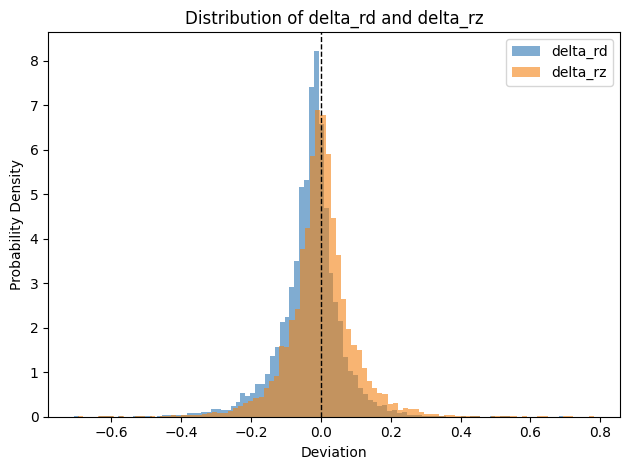
\includegraphics[width=1\linewidth]{figures/delta.png}
    \caption{Distributions of $\delta_{RD}$, numerical deviation of CDNA3 FP16 MFMA instruction that uses the rounding-down (RD) mode, and $\delta_{RZ}$, numerical deviation of a hypothetical FP16 MFMA instruction that uses the rounding-to-zero (RZ) mode.}
    \label{fig:delta}
\end{figure}

These phenomena occur when $A$ and $B$ contain large-magnitude numbers and the elements of $C$ are negative numbers with relatively small magnitudes. We note that AMD has added a patch to CDNA3 FP8 MFMA instructions. As shown in Step 8 of GFDRDA, there is an additional check for the exponent of $c$. If $e_c<e_{max}-25$, then $c$ is rounded to zero instead of rounded down. This patch avoids the cases above.

\textbf{Architectural insight.} We note that if the hardware uses two's complement encoding to store and compute intermediate sums, RD is the most natural choice for rounding because RD can be implemented by simply truncating the least significant bits in two's complement encoding. In addition, if hardware uses ones' complement or sign-magnitude encoding, RZ is the most natural choice because RZ can be implemented by simply truncating the least significant bits in these encodings. Because floating-point numbers are based on the sign-magnitude encoding, we suggest using sign-magnitude arithmetic as well and choosing RZ as the rounding mode.

\textbf{Software insight.} On the CDNA3 architecture, we suggest using Matrix Cores only for matrix multiplication by setting $C=0$, and using the general compute units for full FP32-precision matrix accumulation to mitigate this issue in the TF32, FP16, and BF16 instructions.

\section{Related Work}


Without a standard and consistent arithmetic behavior, matrix multiplication accelerators (MMAs) raise challenges in AI research and development. Deepseek developers \cite{deepseek-ai_deepseek-v3_2024} have reported that the training accuracy of their LLM is significantly degraded due to the insufficient accumulation precision of the FP8 matrix multiplication instructions of the Hopper architecture. This To mitigate the issue, they use additional CUDA Cores to perform full FP32-precision matrix accumulation. PyTorch developers \cite{pytorch_developers_pytorch_2025} have reported that the FP16 and BF16 MFMA instructions of the CDNA2 architecture will flush subnormal numbers to zero, and FP16 DNN training may fail to converge as subnormal values frequently occur during gradient calculation in the backward pass. To mitigate the issue, they cast FP16 to BF16 for computation in the backward pass, which increases the dynamic range but sacrifices precision.

In addition, previous studies have reported numerical inconsistency issues across different hardware \cite{jezequel_estimation_2015}, GPU vendors \cite{zahid_testing_2024}, and different generations of MMAs \cite{li_discovery_2024} due to intricate properties of floating-point arithmetic. Reproducibility of DNNs is an important goal for AI researchers \cite{pham_problems_2020,chen_towards_2022,he_defeating_2025}, but hardware-related numerical inconsistency makes it rather difficult \cite{xie_revealing_2025}.

Although many studies have modeled the arithmetic behavior of existing MMAs, none of them are verified to be bit-accurate. Raihan et al. \cite{raihan_modeling_2019} intuitively model the dot product operation of the Tensor Core as a full binary tree of multiplication and addition operations. However, this is incorrect, as disproved by Hickmann et al. through numerical experiments \cite{hickmann_experimental_2019}. Their numerical experiments indicate several characteristics of the Tensor Core on the Volta architecture. Fasi et al. \cite{fasi_numerical_2021} extend the numerical experiments to the Tensor Cores on the Turing and Ampere architectures, and Li et al. \cite{li_fttn_2024} extend to the Tensor Core on the Hopper architecture and the Matrix Cores on the CDNA1 and CDNA2 architectures. Xie et al. \cite{xie_revealing_2025} invent an algorithm to reveal the floating-point summation order in MMAs. However, these studies only cover a part of the arithmetic behavior of the accelerators, incomplete for a bit-accurate reference model. Moreover, some of their results are incorrect, as reported by Valpey et al.\cite{valpey_smt_2025}. Without bit-level verification, the results of these studies lack reliability.


\section{Conclusion}

This paper introduces MMA-Sim, the first bit-accurate reference model that reveals the detailed arithmetic behaviors of matrix multiplication accelerators (MMAs) from NVIDIA and AMD GPUs. Through systematic testing and large-scale validation, MMA-Sim achieves bitwise equivalence with the real hardware and uncovers many previously undocumented arithmetic behaviors.

MMA-Sim will be open-source, providing a publicly accessible tool for transparent numerical analysis, cross-vendor comparison, arithmetic behavior reproduction, and precision-aware co-design of future accelerators and AI systems.

\appendix
\label{sec:appendix}

\subsection{Floating-point formats for matrix multiplication}
\label{ssec:FPformat}

Floating-point matrix multiplication is one of the most fundamental and dominant operations in numerical computing, high-performance computing, and deep learning. Traditionally, IEEE-754 double-precision (FP64) and single-precision (FP32) formats are most prevalent in software and hardware. FP64 and FP32 matrix multiplication is implemented with standard IEEE-754 arithmetic \cite{ieee_ieee_2019}, i.e., floating-point multiplication and addition, or fused multiply-add (FMA) operation.

As deep neural networks (DNNs) become increasingly popular, the computational efficiency and scalability of floating-point matrix multiplication has become even more critical to modern computer systems. To achieve high efficiency and scalability, recent DNNs, particularly large language models (LLMs), adopt low-precision floating-point formats.

Among the low-precision formats, TensorFloat-32 (TF32), half-precision (FP16) and brain-float16 (BF16) formats use the encoding method similar to the IEEE-754 standard for normal numbers, subnormal numbers, zeros, infinities and NaNs; they just reduce the number of exponential bits and the number of mantissa bits. Other formats have more complexities.

Eight-bit formats (FP8) include four common variants: E5M2, E4M3FN, E5M2FNUZ, and E4M3FNUZ, where E$x$M$y$ indicates $x$ exponential bits and $y$ mantissa bits, and FN and FNUZ denote different special encoding methods (FN has no infinity, and FNUZ has neither infinity nor negative zero). The E5M2 and E4M3FN variants are defined by \cite{micikevicius_fp8_2022,open_compute_project_ocp_2023} and supported by recent NVIDIA GPUs. The E5M2FNUZ and E4M3FNUZ variants are defined by \cite{noune_8-bit_2022} and supported by AMD CDNA3 GPU.

The encoding method of six-bit (FP6) and four-bit (FP4) formats discards support for infinity, negative zero, and NaN. In addition, a group of 32 FP8, FP6, or FP4 numbers can be extended to MXFP8, MXFP6, or MXFP4 formats \cite{open_compute_project_ocp_2023} by multiplying a scale factor shared by all 32 elements. The scale factor is encoded as UE8M0, which can only represent NaN and the power of twos ranging from $2^{-127}$ to $2^{127}$. NVIDIA also supports a variant of MXFP4 by reducing the block size from 32 to 16, and an additional variant called NVFP4 by additionally changing the scale factor format from UE8M0 to UE4M3 (unsigned E4M3FN).

\subsection{Tensor Core instructions}
\label{ssec:TCinst}
NVIDIA GPUs provide warp-level matrix multiply-accumulate instructions (DMMA, HMMA, QMMA, and OMMA) to perform the matrix multiply-add operation (Equation \ref{eq:mm}) with Tensor Cores. In addition, the Hopper architecture provides warp-group-level matrix multiply-accumulate instructions (HGMMA and QGMMA), and the Blackwell architecture provides warp-group-level/warp-group-pair-level matrix multiply-accumulate instructions (UTCHMMA, UTCQMMA, and UTCOMMA). All these Tensor Core instructions and their compatability are listed in Table \ref{tab:nvmodel}.

These Tensor Core instructions support a large number of data types and shapes, which are indicated by the instruction names (except the UTCHMMA, UTCQMMA, and UTCOMMA instructions, whose type and shape information are stored in an instruction descriptor data structure). The shapes of the matrices are indicated by \textit{MNK} or \textit{M}x\textit{N}x\textit{K}. For example, ``16816'' or ``16x8x16'' means that $M=16$, $N=8$, and $K=16$.

For DMMA instructions, the data types of $A$, $B$, $C$, and $D$ are double-precision (FP64).

For HMMA and HGMMA instructions, the data types of $A$ and $B$ must be the same. The specific data types are indicated by the instruction suffix as shown below.
\begin{itemize}
    \item ``.F32.TF32'' means that $A$ and $B$ are TF32, and $C$ and $D$ are FP32.
    \item ``.F32.BF16'' means that $A$ and $B$ are BF16, and $C$ and $D$ are FP32.
    \item Otherwise, $A$ and $B$ are FP16.
    \begin{itemize}
        \item ``.F32'' or ``.F32.F32'' means that $C$ and $D$ are FP32.
        \item ``.F16'' or ``.F16.F16'' means that $C$ and $D$ are FP16.
        \item ``.F32.F16'' means that $D$ is FP32 and $C$ is FP16.
    \end{itemize}
\end{itemize}
HMMA.884 instructions are special because one instruction can perform four concurrent $8\times 8\times 4$ matrix multiplications simultaneously. Other instructions only perform one $M\times N\times K$ matrix multiplication operation.

For QMMA and QGMMA instructions, the data types of $C$, $D$, $A$, and $B$ are indicated by ``\textit{.cdtype.atype.btype}''. $A$ or $B$ can be any FP8 data type (E4M3 or E5M2), or any FP8, FP6, or FP4 data type (E4M3, E5M2, E2M3, E3M2, or E2M1) on the RTX Blackwell architecture. NVIDIA uses E4M3 to represent the E4M3FN encoding for FP8. The data types of $C$ and $D$ must be the same and can be FP32 or FP16. 

QMMA.SF instructions support MXFP8, MXFP6, and MXFP4 data types. Specifically, indicated by ``\textit{.cdtype.atype.btype.sftype}'', $C$ and $D$ are FP32, $A_{M\times K}$ and $B_{K\times N}$ are FP8, FP6, or FP4, and the scale factors $A^{SF}_{M\times (K/32)}$ and $B^{SF}_{(K/32)\times N}$ are UE8M0. Each output element is computed as
\begin{equation}
\label{eq:mxfpmm}
d_{ij}=c_{ij} + \sum_{k=0}^{K-1}a_{ik}a^{SF}_{i\lfloor k/S \rfloor}b_{kj}b^{SF}_{\lfloor k/S \rfloor j}
\end{equation}
where $S=32$ is the block size.

Similarly, the OMMA.SF instruction with the ``.F32.E2M1.E2M1.E8'' suffix supports MXFP4 input. In addition, the OMMA.SF instruction with the ``.F32.E2M1.E2M1.UE4M3.4X'' suffix supports NVFP4 input, where the scale factors $A^{SF}_{M\times (K/16)}$ and $B^{SF}_{(K/16)\times N}$ are UE4M3 and the block size $S$ is 16 instead of 32.

Blackwell-specific instructions support similar data types and more matrix shapes in terms of $M$ and $N$. Specifically, UTCHMMA supports the data type combinations same as HGMMA, with $K=8$ for TF32 and $K=16$ for FP16 and BF16. UTCQMMA supports data type combinations same as QMMA and QMMA.SF on RTX Blackwell, with $K=32$ and optional scale factors of block size $32$. UTCOMMA and UTCOMMA.X4 support the same data types as OMMA.SF instructions, with $K=64$ and the block size being 32 or 16.

\subsection{Matrix Core instructions}

Recent AMD GPUs provide warp-level matrix fused-multiply-add (MFMA) instructions to perform the matrix multiply-add operation (Equation \ref{eq:mm}) with Matrix Cores. At the time of writing, we do not have a CDNA1 GPU, so this paper only covers the CDNA2 and CDNA3 architecture and leaves CDNA1 for future work. We list their Matrix Core instructions in Table \ref{tab:amdmodel}.

For CDNA2 MFMA instructions, the shape and type information is indicated by instruction names in format v\_mfma\_\textit{cdtype}\_\textit{M}x\textit{N}x\textit{K}\textit{abtype}. Some BF16 instructions have a ``\_1k'' suffix to distinguish from legacy BF16 instructions inherited from CDNA1.

CDNA3 renames the instructions in format v\_mfma\_\textit{cdtype}\_\textit{M}x\textit{N}x\textit{K}[\_\textit{T}b]\_\textit{abtype}, where \textit{abtype} can be \textit{atype\_btype} for FP8 instructions, and $T$ means the number of concurrent matrix multiplications executed by one instruction (CDNA2 also does so but omits this information in its instruction names). AMD uses xf32 to represent TF32, fp8 to represent E4M3FNUZ, and bf8 to represent E5M2FNUZ.


% \bibliographystyle{ACM-Reference-Format}
\bibliographystyle{IEEEtran}
\bibliography{references}

\end{document}
